\documentclass{bioinfo}
\usepackage{multirow}
\usepackage{comment}
\usepackage{placeins}
\usepackage{color}
\usepackage[T1]{fontenc}
\copyrightyear{2014}
\pubyear{2014}

\begin{document}
\firstpage{1}

\title[fastPSSM]{Fast generation of PSSMs.}
\author[Shu \textit{et~al}]{Nanjiang Shu\,$^{1,2}$ ,Stefano
  Pascarelli $^{1}$, Christoph Peters\,$^{1}$,  Konstantinos D. Tsirigos\,$^{1}$, 
Walter Basile\,$^{1}$ and Arne Elofsson\,$^{1}$\footnote{to whom correspondence should be addressed}}
\address{$^{1}$Department of Biochemistry and Biophysics, Science for
  Life Laboratory,Stockholm University,
Box 1031, 17121 Solna, Sweden,
$^{2}$Sweden Bioinformatics Infrastructure for Life Sciences (BILS), Stockholm University, Sweden.}
\history{Received on XXXXX; revised on XXXXX; accepted on XXXXX}

\editor{Associate Editor: XXXXXXX}

\maketitle

\begin{abstract}
  \section{Motivation:}
  Generation of PSSM growing datase

    \section{Results:}  On average X procent of the time can be soend
So far we have used earlier versions of fastPSSM in the TOPCONS
webserver. In total more than 4.5 million PSSMs has been
generated. The average running time has been about 1 minute. This
corresponds to an approximate 10 times speedup.

  \section{Availability and implementation:}

 github...

  \section{Contact:}
  \href{mailto:arne@bioinfo.se}{arne@bioinfo.se}
\end{abstract}

% \vspace{-.5cm}
\section{Introduction}


Sequence searching is the fundament that almost all bioinformatics
tools rely on. Therefore, fast and sensitive algorithms are
crucial. Throughout history the introduction of better and faster
algorithms, such as blast~\cite{}, psiblast~\cite{Altschul},
hhblits~\cite{soding} and hmmer3~\cite{eddy} has during the last 20
years enabled detection of homologs in the entire uniprot database
using a single computer in a few minutes. However, these methods are
too slow to apply to easily apply to the entire database (requires
$N^2$ searches) or for mapping short reads.

Since the beginning in the 1970's it has been a consistent battle
between the growth of databases and the increase in computer
speed. The introduction of next generation sequences clearly showed
that the size of the databases was growing faster than computer speed,
indicating that searching the complete database will be slower and
slower. 

For many applications the availability of a position specifiv scoring
matrix (PSSM) or a hidden Markov model (HMM) for a protein is
needed. These are calculated from a multiple sequence alignmetns and
can drastically improve secondary structure~\cite{phd} and many other type of
predictions~\cite{TOPCONS}.


Many attempts have been made to obtain faster searches than the best
sequence search methods without loosing in
performance~\cite{hhblits,deltablast,berger}. However, to the best of
our knowledge they do either loose in sensitivity or the speedup is
just linear. 

Here we propose a simple tool that gains on average close to one order
of magnitute in improvement without an loss in sensitivity. In short
the idea is very similar to what is used in deltaBlast, i.e. a first
search is performed against a several order of magnitude domain
database. However, in contrast to deltaBlast we do not stop after this
search, instead we extract the full length sequences of all to create
an intermediate database, Figure~\ref{fig:foobar}a.

We have used an earlier verion of this tool for the last year in the
TOPCONS webserver for generating PSSMs for several million of
sequences.


EARLIER WORK 

alternative methods.


\section{Methods}





 %\vspace{-.0cm}

\section{Results and Discussion}


\begin{figure*}[t]
  \resizebox{0.45\textwidth}{!}{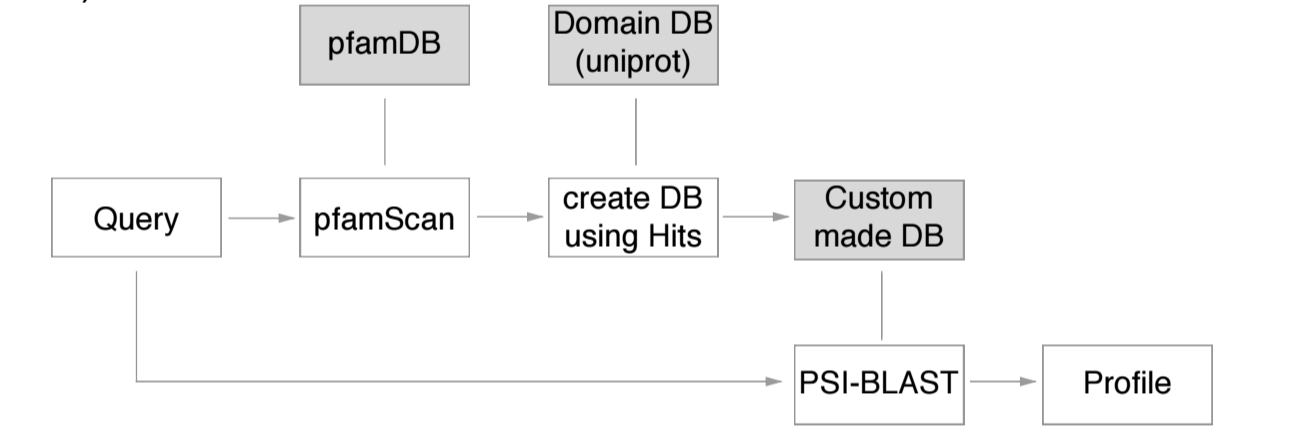
\includegraphics{workflow.png}}\\
  \resizebox{0.45\textwidth}{!}{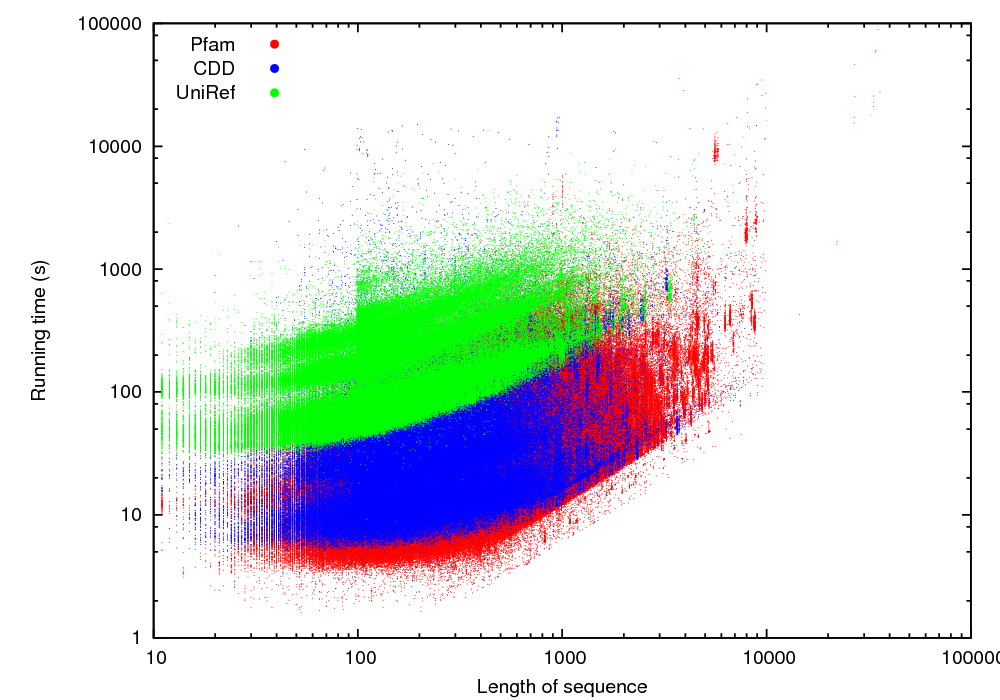
\includegraphics{length_runtime.png}}
\label{fig:foobar}
 \caption{a) Workflow. b) Running time for different sequences in TOPCONS2~\cite{Tsirigos25969446}}
\end{figure*}



% \vspace{-.5cm}
\section{Conclusions}

{\footnotesize
% \vspace{-.5cm}

\section*{Acknowledgement}
\paragraph{Funding}
\footnotesize{This work was supported by grants from the Swedish
  Research Council (VR-NT 2012-5046). NS was financed by
  Bioinformatics Infrastructure for Life Science (BILS).}
%\vspace{-.5cm}

\bibliographystyle{natbib}
\bibliography{refs}
%\begin{thebibliography}{}
\end{document}

\end{document}
